\documentclass[10pt,a4paper]{article}
%\usepackage[utf8]{inputenc}
\usepackage{amsmath}
\usepackage{amsfonts}
\usepackage{amssymb}
\usepackage{graphicx} %For images
\usepackage[german]{babel}

\usepackage{listings} %For code

\begin{document}

%Titelseite
\begin{titlepage}

\begin{center}
\vspace*{1.3cm}
{\Huge Dependable Systems\\(VU 182.712)\\}
\vspace{1.7cm}
{\LARGE Praktisches Ubungsbeispiel SS2015:\\``Zuverl�assigkeitsmodellierung mit \textit{sharpe}''\\}
\vspace{1.7cm}


{\hspace{1cm} Datum der Labor�bung: 18.06.2015}


\begin{table}[h!]
\centering
\begin{tabular}{|p{3.5cm}|p{6.5cm}|}
\hline \textbf{Matr. Nr.} & \textbf{Name} \\
\hline
1228774 &  Schieber Constantin \\
\hline
&  Pacheiner Peter \\
\hline
1226314 & Hofer David \\
\hline
\end{tabular}
\end{table}

\end{center}
\vspace{1.0cm}

\end{titlepage}
\setcounter{page}{2}






\newpage
\section{Abstract}
Ein Computernetzwerk soll durch Markovketten modelliert werden um es auf Fehlersicherheit zu überprüfen.
\\ 
Konkret soll die Mean Time to Failure (MTTF) und die Verfügbarkeit zwischen 2 Systemen evaluiert und verglichen werden. Eines ohne Redundanz und eines mit.
Zusätzlich soll ein Vergleich zwischen den Kosten fuer die beiden Systeme durchgeführt werden.
\section{Aufgabenstellung}
Für beide Systeme gelten die folgenden Fehlerraten ($\lambda$) und Reparaturraten ($\mu$).
\begin{itemize}
	\item $\lambda_R=10^{-4}/Std.$ fuer Rechner
	\item $\lambda_N=2*10^{-5}/Std.$ fuer Switches
	\item  $\mu=10^{-2}/Std. $
	
Um funktionsfaehig zu sein benoetigt das Netzwerk mindestens einen Switch und drei Rechner.
\end{itemize}
\section{Mean Time to Failure}
\subsection{Einfaches System}
Das Computernetzwerk besteht aus drei über einen Switch verbunden Rechnern.
\\
Um die MTTF zu evaluieren reicht es das System durch 2 Zustaende zu modellieren. \\
Einer stellt den funktionierenden Zustand (0) dar, der andere den Fehlerzustand (1).
Die Wahrscheinlichkeit fuer einen Uebergang in den Fehlerzustand setzt sich dann aus $3*\lambda_R + \lambda_N$ zusammen. Diese Vereinfachung kann vorgenommen werden da jeder Ausfall, egal welcher Art, in einen Fehlerzustand fuehrt. 
Die Reparaturrate muss nicht berücksichtigt werden da wir uns im Moment ausschließlich fuer die MTTF interessieren.
\\
Das System kann sowohl graphisch als auch in Textform beschrieben werden:
\begin{figure}[ht!]
\centering
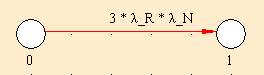
\includegraphics[width=90mm]{MTTM_EinfachesModell.png}
\caption{Einfaches System in \textit{sharpe} modelliert \label{mmtm_einfach}}
\end{figure}

\lstinputlisting{MTTF_Einfach_Modell.txt}
\subsection{Redundantes System}
Das redundante Computernetzwerk besteht aus 4 Rechnern und 2 Switches was die Ausfallwahrscheinlichkeit gegenueber dem einfachen System deutlich verringern sollte.\\
Statt 2 Knoten werden nun 5 Knoten benoetigt um alle Uebergaenge korrekt abzubilden.\\
Das System ist in den Knoten 0,1,2,3 funktionsfaehig, Knoten 4 ist der Fehlerzustand (siehe Grafik \ref{mmtm_redundant}).
\begin{figure}[ht!]
\centering
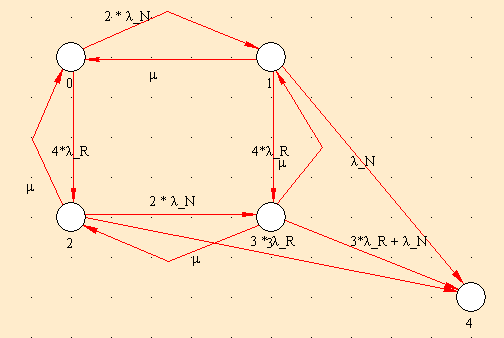
\includegraphics[width=90mm]{MTTM_ReduntantesModell.png}
\caption{Redundantes System in \textit{sharpe} modelliert \label{mmtm_redundant}}
\end{figure}
\lstinputlisting{MTTF_Redundant_Modell.txt}
\subsection{Vergleich der beiden Systeme}
Um die beiden Systeme vergleichen zu koennen muss nun auch die Simulation derselbigen durchgeführt werden. Dies geschieht durch folgende Befehlssequenz in \textit{sharpe}:
\lstinputlisting{MTTF.txt}

Daraus resultieren die folgenden Ergebnisse: 
\lstinputlisting{MTTF_RESULTS.txt}
Das bedeutet dass das einfache Modell nach ca. 31250 Stunden ausfällt und das redundante erst nach 88540 Stunden. Man sieht dass sich durch das hinzufügen der Redundanz der Zeitraum bis zum Ausfall deutlich erhoeht. 
\section{Availability}
Im Gegensatz zur MTTF ist bei der Availability die Reparaturrate nun auch vom Fehlzustand aus zu berücksichtigen.
\subsection{Einfaches System}
Für das einfache System wird einfach eine neue Kante die zurueck in den funktionierenden Zustand fuehrt hinzugefuegt.
\begin{figure}[ht!]
\centering
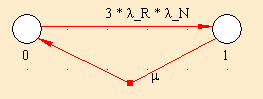
\includegraphics[width=90mm]{AVAILABILITY_Einfach.png}
\caption{Einfaches System mit neuer Kante in \textit{sharpe} modelliert \label{avail_einfach}}
\end{figure}
\lstinputlisting{AVAILABILITY_Einfach.txt}
\subsection{Redundantes System}
Im redundanten System reicht nun ein Fehlerzustand nicht mehr aus da wir aus diesem auch wieder zurueck kehren koennen. Um sich den Zustand des restlichen Systems zu "merken" bzw. um deterministisch agieren zu koennen werden 3 neue Knoten eingefuehrt, die jeweils als Fehlzustaende fungieren und ueber eine Kante mit dem letzten funktionierenden Zustand verbunden sind. 
\begin{figure}[ht!]
\centering
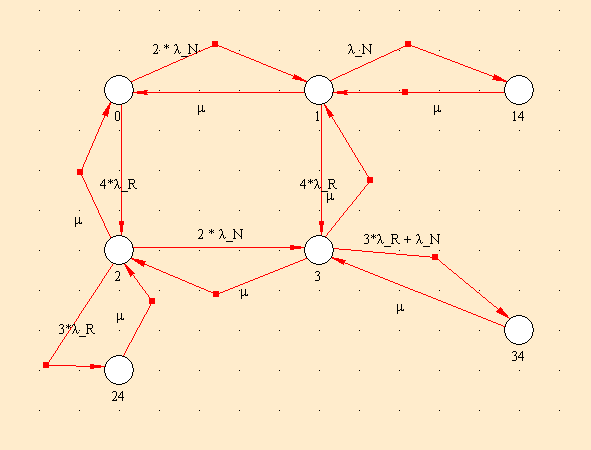
\includegraphics[width=90mm]{AVAILABILITY_RED.png}
\caption{Redundantes System mit neuen Knoten und Kanten in \textit{sharpe} modelliert \label{avail_einfach}}
\end{figure}
\lstinputlisting{AVAILABILITY_RED.txt}
\subsection{Vergleich der beiden Systeme}
Der Vergleich der beiden Systeme wird mit dem Befehl \textit{prob(SYS, NODE)} ausgeführt. Dieser errechnet die Zustandswahrscheinlichkeit fuer eine bestimmte \textit{NODE} im angegebenen System.\\
Im einfachen System reicht es die Wahrscheinlichkeit berechnen zu lassen mit der sich das System im gültigen Zustand befindet. \\
Im redundanten Fall ist es einfacher die Wahrscheinlichkeit der Fehlzustände berechnen zu lassen, diese zu addieren und von 100\% abzuziehen.
Der Aufbau der Befehlsabfolge sieht so aus:
\lstinputlisting{AVAILABILITY.txt}
Und das Ergebnis dann folgendermaßen:
\lstinputlisting{AVAILABILITY_RESULTS.txt}
Wie man sieht beträgt die Wahrscheinlichkeit dafür dass sich das einfache System in einem gültigen Zustand befindet $96.899\%$. \\
Die Wahrscheinlichkeit in einem redundanten System beträgt dafür $99.87\%$.
\section{Kosten}
\end{document}